\section{Plotting the band structure and density of states of a solid}
\label{band and dos plotting}

An example for plotting band structures and the
density of states is contained in the example for bulk silicon (diamond
lattice) in the testcases directory. Likewise, the fcc Al test case contains 
the necessary lines for control.in (just commented out).

This
section contains a walk-through of the necessary steps and keywords to
obtain this band structure and density of states. First, let us look
at the relevant lines in \texttt{control.in} as given in the test case.

\small
\begin{verbatim}
# output DOS
  output dos -18.  0.  200  0.05
  dos_kgrid_factors 8 8 8

# output band structure
  output band 0.5   0.5   0.5    0.0   0.0   0.0    50  L     Gamma
  output band 0.0   0.0   0.0    0.0   0.5   0.5    50  Gamma X
  output band 0.0   0.5   0.5    0.25  0.5   0.75   50  X     W
  output band 0.25  0.5   0.75   0.375 0.375 0.375  50  W     K
\end{verbatim}
\normalsize

To get an output of the band structure, use the keyword \keyword{output}
\subkeyword{output}{band}. Each '\subkeyword{output}{band}' line
covers a single line in reciprocal space, from a starting point to an
end point and with a given number of points inbetween.

The total density of states of the system is obtained by the
'\keyword{output} \subkeyword{output}{dos}' line, from a starting 
single-particle energy to an ending single-particle energy, with a
specified number of points inbetween and for a given broadening to
create a smooth line (see section \ref{section output} for details).

The density of states of a solid is a continuous function, but
originates from a Brillouin zone integral, 
\begin{equation}\label{Eq:DOS}
  g(\epsilon) = \sum_n \int_\text{BZ} d^3k \, \delta (\epsilon -
                                   \epsilon_n(\boldk)) \, .
\end{equation}
The index $n$ runs over all bands, and $\boldk$ is the crystal momentum.

As it stands, this expression for the density of states creates a
problem. We obtain it from a discrete set of k-points, rather than as
a continuous integral. The density of states from a discrete $k$-mesh
would thus be a sequence of $\delta$-function peaks.

In practice, the $\delta$ function is replaced by a Gaussian function
with a finite width. The chosen width in our test case is 0.05 eV
(typically, 0.1~eV would also be acceptable, although giving a
somewhat more washed-out density of states). 

If we just applied our expression Eq.~\ref{Eq:DOS} to a $k$-space mesh
typically used to obtain a reasonably converged total energy in an
s.c.f. calculation (in our example, '\keyword{k\_grid} 12 12 12'),
horrible things would happen to our DOS. With the broadening chosen
here, a rather wiggly line would result. It turns out that, e.g., a 
'96 96 96' $k$-mesh would yield a much nicer result ... except that
this choice would make any s.c.f. calculation extremely expensive.

What to do?

Here is where the '\keyword{dos\_kgrid\_factors}' line comes in. The
factors given here mandate a the use of a denser $k$-space mesh
\emph{only} for the evaluation of the density of states, after the
s.c.f. calculation is already complete. The effective $k$-mesh used in
our example is 'k\_grid($i$)$\cdot$dos\_kgrid\_factor($i$)' ($i$=1,2,3),
in our case 12$\cdot$8=96 in each direction. However, the extra $k$-points
are only evaluated for the fixed self-consistent Kohn-Sham potential
that emerged from the original s.c.f. calculation.

With the lines for band structure output, DOS output and
\keyword{dos\_kgrid\_factors} in \texttt{control.in}, we can run the
example calculation in the testcases directory.

Once this is done, a number of new files have appeared (in addition to
the usual standard output stream): The files \option{band1XXX.out},
\option{KS\_DOS\_total.dat}, and \option{KS\_DOS\_total\_raw.dat}. 

\begin{figure}
\begin{center}
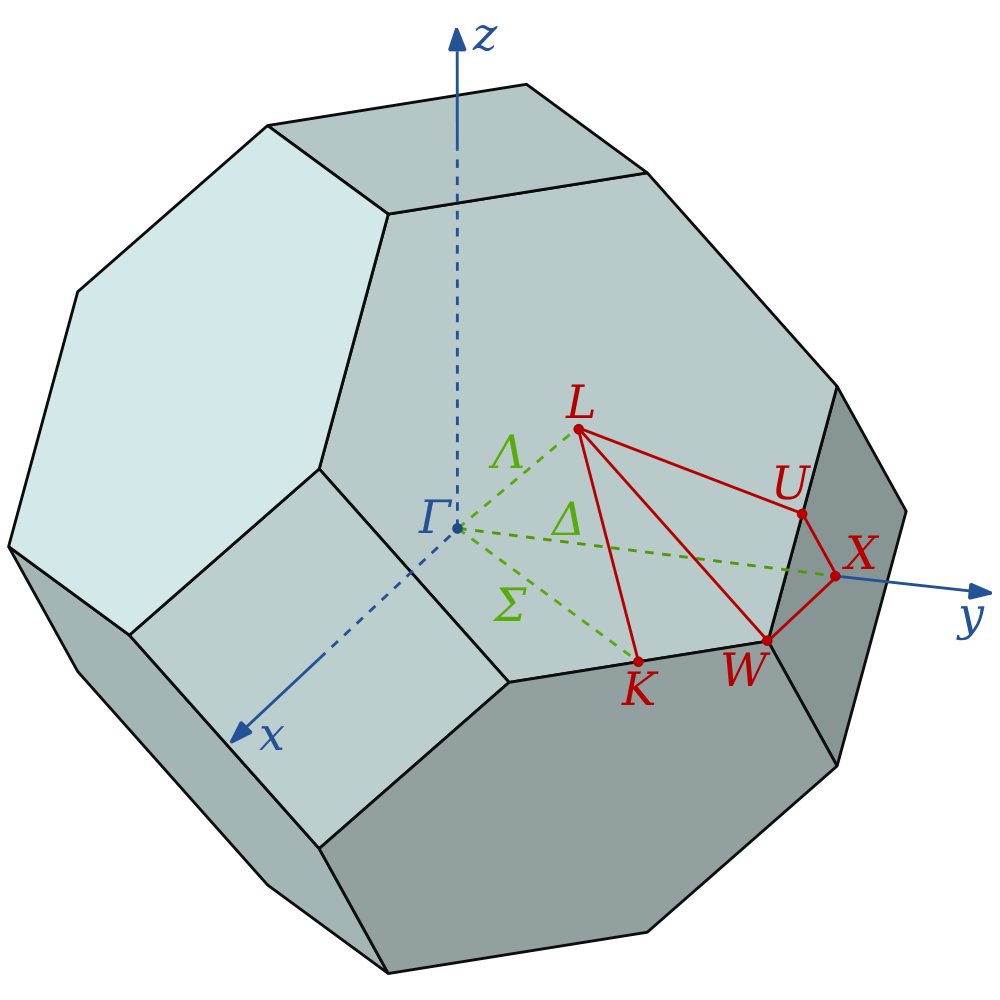
\includegraphics[height=4 cm]{fcc_Brillouin_zone.png}
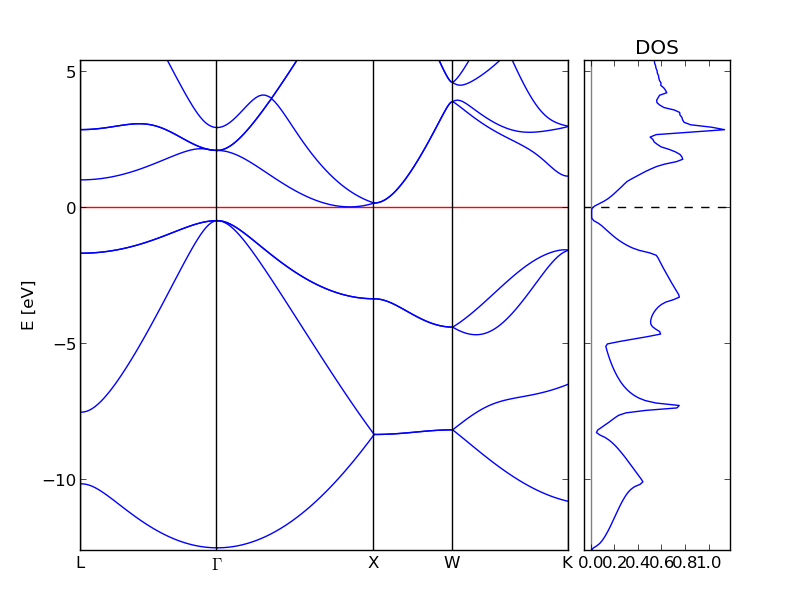
\includegraphics[height=9 cm]{Si_band_structure_and_DOS_reference}
\end{center}
\caption{Band structure and density of states of the bulk Si test case
         as generated by the 'aimsplot.py' script, which is located in the ``utilities''
         directory. A schematic visualization of the Brillouin zone of
         the fcc Bravais lattice including some high-symmetry $k$-points is
         also shown (taken from Wikipedia).} 
\label{band structure figure}
\end{figure}

These files contain the necessary information in column formats that
can be manipulated for further output with standard plotting
tools. The result of such a manipulation is shown in Fig. \ref{band
  structure figure}. 

However, it would be nice to not have to personally massage the output
data every time to get this kind of output. The script 'aimsplot.py',
located in the utilities directory, should do this for you. Simply run
it in the output directory, and a nice-looking band structure and DOS
should automatically appear. 

As there are various conventions for plotting the density of
states, each possible DOS plot produces two different output
files. The first one, ending in ``\_raw.dat'', contains the exact 
density of states, using exactly the  
same eigenvalue energies and energy zero as internally in FHI-aims (in cluster
systems, the energy zero is simply the vacuum level; in periodic systems, the
energy zero is set by the $\boldG$=0 component of the long-range electrostatic
potential). 

The file \option{KS\_DOS\_total.dat} contains
the same information, but the energy zero is shifted to the
Fermi-level of the system. Note that, for metals, the Fermi level is
usually well defined. For insulators, it is not well defined, and may
end up anywhere in the gap (at some location where FHI-aims finds the
normalization criterion for the number of electrons to be sufficiently
fulfilled).

If, for a semiconductor, you wish to have the energy zero of a DOS
shifted to the top of the valence band, you will have to do this as an 
extra step. Identify the location of the valence band edge (highest
occupied level) either from the FHI-aims output or from the band
structure, and shift the x-axis of \option{KS\_DOS\_total.dat} and
other files by the appropriate amount. 

Except for the \emph{total} density of states, there are also a few
other options to obtain densities of states with some local, spatial
resolution. In particular:
\begin{itemize}
  \item an atom-projected density of states, using \keyword{output}
    \subkeyword{output}{atom\_proj\_dos}
  \item an angular-momentum component projected density of states
    averaged over all atoms \emph{of a single species}, using the
    keyword \keyword{output} \subkeyword{output}{species\_proj\_dos}
    . This is useful because different 
    atoms of the same element may be grouped together as a separate
    species in \texttt{control.in}, e.g., all atoms in the first layer
    of a slab.
\end{itemize}

Note that there are two useful projections of the DOS, both of which are based
on a Mulliken analysis. \keyword{output}
\subkeyword{output}{species\_proj\_dos} can be used to  
get a species-dependent angular momentum projection, while
\keyword{output} \subkeyword{output}{atom\_proj\_dos} resolves the
states into the various  
atomic angular-momentum contributions.

As mentioned above, the \subkeyword{output}{species\_proj\_dos} keyword can also be used
to get the DOS contribution from a whole group of atoms at once. Just
duplicate the species defaults for the element(s) in question in
\texttt{control.in}, give the species a new name, and then use that
new species (say) for all surface atoms in \texttt{geometry.in}. This
will get you the density of states contribution from all surface atoms.


% For emacs:
%%% Local Variables: 
%%% mode: latex
%%% TeX-master: "FHI-aims"
%%% End: 
